%% Edited with emacs (set-keyboard-coding-system 'utf-8)
%% COMPILATION: pdflatex -synctex=1 -interaction=nonstopmode escad_manual.tex
%% COMPILATION WITH EXTERNAL-PACKAGE: pdflatex -synctex=1 -interaction=nonstopmode --shell-escape escad_manual.tex
%% COMPILATION ALTERNATIVE: latexmk -pdf escad_manual.tex
%% Emacs-modes: latex-mode, outline-minor-mode
%% Emacs-commands: M-x outline-toggle-children
%% M-x pdf-tools-install
%% M-x customize apropos TeX-source-correlate-method -> synctex
%% M-x TeX-source-correlate-mode
\documentclass[a4paper, 12pt, openany]{scrbook}
\usepackage[T1]{fontenc}
\usepackage{lmodern,textcomp} % Euro symbol
\usepackage[utf8]{inputenc}  % umlauts (without \"a)
% \usepackage[ngerman]{babel}  % new german rules
\usepackage[UKenglish]{babel}  % english for toc...
\usepackage[paper=a4paper, left=2cm, top=20mm, bottom=15mm, right=15mm, includefoot, foot=\baselineskip, footskip=10mm]{geometry} % borders
\usepackage[headsepline,footsepline]{scrpage2}
%\usepackage{longtable}
\usepackage[table]{xcolor}
\usepackage{amsmath}
\usepackage{rotating}
\DeclareMathOperator\sign{sign}
\usepackage{listings}
\usepackage[autostyle]{csquotes} % Anführungszeichen mit \enquote{Anführungszeichen}
%\usepackage{tikz-timing}[2009/05/15]
%\lstset{basicstyle=\scriptsize} 
\lstset{basicstyle=\footnotesize\ttfamily, numbers=left, numberstyle=\tiny\color{blue}, frame=single, firstnumber=1, keywordstyle=\color{blue}}
%\lstset{basicstyle=\small} 
\lstset{literate=%
    {Ö}{{\"O}}1
    {Ä}{{\"A}}1
    {Ü}{{\"U}}1
    {ß}{{\ss}}1
    {ü}{{\"u}}1
    {ä}{{\"a}}1
    {ö}{{\"o}}1
    {~}{{\textasciitilde}}1
    {°}{{\textdegree}}1
}
\usepackage{upgreek} % uppright (mathly correct) pi in math-mode
\usepackage[locale=DE,per=frac]{siunitx}
\usepackage{amssymb} %für Mathesymbole wie Menge der natürlichen Zahlen
%\usepackage{color} % farbiger Texthintergrund
\usepackage{xcolor} % Text color
%\usepackage{pdfpages}
%\usepackage[abs]{overpic}
%\usepackage{lastpage} % für gesamtseitenzahl
\usepackage{tikz} % graphical drawing
\usepackage{pgfplots}
\usetikzlibrary{matrix, positioning, shapes}
\usetikzlibrary{arrows, automata, shadows, patterns}
% \usepackage{circuitikz}
%\usetikzlibrary{external} % faster compilation, but see compile command
%\tikzexternalize[prefix=figures/] % activate and define figures/ as cache folder
\usepackage{index}
\makeindex
\pagestyle{scrheadings}

\clearscrheadings
\clearscrheadfoot
\newcommand{\MyVorname}{Markus}
\newcommand{\MyNachname}{Kollmar}
\newcommand{\EscadVersion}{0.1}
\newcommand{\MyTitel}{Manual for ESCAD version \EscadVersion}
\newcommand{\MyDate}{\today}
\ohead{page: \pagemark}
%\chead{Lösung}
\ihead{\MyTitel}
\ofoot{\MyVorname\, \MyNachname}
%\cfoot{}
\ifoot{\MyDate}

\usepackage[pdftex,
            pdfauthor={Markus Kollmar},
            pdftitle={\MyTitel},
            pdfsubject={\MyTitel},
            pdfkeywords={manual},
%            pdfproducer={Latex with hyperref},
%            pdfcreator={pdflatex}
]{hyperref}  % Metadaten in PDF

\author{\MyVorname \quad \MyNachname}
\title{\MyTitel}


\input{kvmacros}

%% command-reference function {cmd-name}{input}{output}{description}:
\newcommand{\escadcmd}[4]{\index{command reference!#1}
  \colorbox{black!20}{\parbox[c][1em]{160mm}{\texttt{#2}}}\\
  \colorbox{green!20}{\parbox[c][1em]{160mm}{\texttt{#3}}}\\#4}

%% shell command-line {cmd-name}{result}:
\newcommand{\shellcmdline}[2]{\\
  \setlength{\fboxsep}{2pt}\colorbox{black!20}{\parbox{\textwidth}{\texttt{user@host:$\sim$/escad\$ \textbf{#1}\\#2}}}\\}

%% escad command-line {cmd-name}{result}:
\newcommand{\escadcmdline}[2]{\\\setlength{\fboxsep}{2pt}\colorbox{black!20}{\parbox{\textwidth}{\texttt{ESCAD> \textbf{#1}\\#2}}}\\}

%% lisp command-line {cmd-name}{result}:
\newcommand{\lispcmdline}[2]{\\\setlength{\fboxsep}{2pt}\colorbox{black!20}{\parbox{\textwidth}{\texttt{> \textbf{#1}\\#2}}}\\}

%%%%%%%%%%%%%%%%%%%%%%%%%%%%%%%%%%%%%%%%%%%%%%%%%%%%%%%%
\begin{document}

\begin{titlepage}
   \begin{center}

     %\vspace*{1cm}
     
     {\huge \MyTitel \ - \MyDate}

     \vspace{0.5cm}

     {\small by:\ \MyVorname\ \MyNachname}

     \vspace{0.5cm}
     
     \begin{tikzpicture}
       \coordinate(front)at(0,0);
       \coordinate(horizon)at(0,.41\paperheight);
       \coordinate(bottom)at(0,-.6\paperheight);
       \coordinate(sky)at(0,.47\paperheight);
       \coordinate(left)at(-.41\paperwidth,0);
       \coordinate(right)at(.41\paperwidth,0);
       \shade[bottom color=white,top color=blue!40!black!50]([yshift=-120mm]horizon-|left)rectangle(sky-|right);
       \node[circle, fill=orange!30] (user) at (0,12) {USER};
       \node[circle, fill=green!20] (escad) at (0,0) {ESCAD};
       \node[circle, fill=green!20] (world) at (-4,7) {WORLD};
       \node[circle, fill=green!20] (view) at (3,5) {VIEW};
       %\draw [thin, gray,-latex] (escad) -- (user);
       \draw [gray] (escad) to [out=50,in=195] (user);
       \draw [red] (escad) to [out=-120,in=165] (world);
       \draw [yellow] (escad) to [out=-60,in=20,looseness=2.2] (view);

       \draw [blue!60] (user) to [out=0,in=20,looseness=2.2] (view);
       \draw [green!60] (user) to [out=140,in=100] (world);
       \draw [red!60] (world) to [out=0,in=100] (view);
     \end{tikzpicture}

     
     \vfill
            
      Alles hängt mit allem zusammen. Wir haben nur nicht das ganze Bild...
            
       \vspace{0.8cm}

     \end{center}
\end{titlepage}


%\maketitle
%\pagebreak
%\cleardoublepage
\tableofcontents
%\pagebreak

\chapter{Introduction}
First of all i have have to apologize that escad and this manual is not in a mature state. There is much to develop and to do. So some things may not work as expected, look different than documented, or there are silly mistakes around. But i think it is better to regularly update the system and documentation, than work some month and there is no regularly progress visible. Documentation lives like the code! I recommend - and think it is very useful - to \textbf{read this manual}. Because you get a feeling about escad and its terminology. And unlike other manuals, escad tries a documentation-driven development process, which will be explained in the next section. This makes this documentation a view of the current development and shows you what can be awaited from escad and what not.
\section{Documentation-driven development (why this manual)}
Documentation-driven development means here (at least we try), at first we define in this manual what we want to develop, and how it looks for the user. Then the feature will be implemented after this specification. Thus we are forced to think more like what a user want, than what is more convenience for the developer. This is an advantage for the user, since he can see what a feature will look like, and documentation is mostly ahead and not behind the actual implementation. The specified feature in the manual, align to the mentioned version of escad. If some feature will be in a later version, this should be mentioned by a version notice.
All follows this process in short:
\begin{enumerate}
\item Set version
\item Update/create documentation (manual)
\item Develop along documentation
\item Test
\item Deliver version (or tag it)
\end{enumerate}
\section{Philosophy (why escad arised)}
History tells us about separation. Separation between different professions was and is common. People have different interests and different knowledge. So this seems natural. Is this a problem? No. And yes. Nowadays science goes into a direction where \textbf{interdisciplinarity} seems more useful. The bounds of our disciplines are drawn by human but it not need to reflect the reality in nature. Real problems are mostly system-problems. Systems are combined of different disciplines. But do the (software) tools support this fact? Some may but many do not. This seems not a big problem in many cases. But when it comes to documentation or knowledge transfer tasks, this can be a big problem. The tools often do not interact with each other, and if so they often feel not integrated well. This problem increases when different manufacturers have tools which interact not or very bad.

Living in todays world is getting more and more complex. There are laws made by human which you have to obey. Additionally mother nature has their ever-lasting rules, overwriting all human rules, and which we should obey to keep the environment healthy for future mankind. Thus people may have the need to get information about this \index{complexity}\textbf{complex} system and tools to make this understandable. Escad is not good in some things. In fact it is really not yet a good graph analysis tool (however one could update that functionality). Escad wants to be a (relatively simple) worker which allows combining different domains in one model: get something out of your semantic-graph-model, avoid switching different tools too much, make \LaTeX\ , PDF, 3D models, music or other documents, which would be boring to create by hand. You can additionally also use the \textbf{scripting} facility of escad.
\section{State (what happens currently)}
Currently escad is in (wild) development. This means there are many ideas which should be developed. Some are just a quick hack to show what is possible and some are more detailed. However but only usable for experts in some areas. Many things are not completed. This is often to just give the idea what should come and is intended to be completed later if the system interacts satisfactorial as a whole.
Future plans are (among many other things not mentioned):
\begin{itemize}
\item Increase domain functionality with practic use.
\item Create good and clear documentation with examples.
\item Make a good graphical user interface in browser via REST-interface.
\end{itemize}
Escad use open interfaces and provide a wide variety of different domain tools. And if there is (yet) not the thing you need, you can customize Escad with common-lisp code. Escad wants to be kind and helpful to the user. \textbf{Your help is really welcome}: if you want maintain this manual, increase escad features, write expansions, create logo, manage homepage or just send some feedback - all things are kind to start a escad-community. Currently the best way to use escad is the terminal, or use the emacs editor, like in figure~\ref{fig:escad_emacs} where you can type in escad-lisp commands.
\begin{figure}[htbp]
  \centering
  \begin{tikzpicture}[node distance=0.6cm and 1cm]
    \node[anchor=south west] (escad_emacs) at (0cm,0cm) {\includegraphics*[scale=0.35]{escad_emacs.png}};
  \end{tikzpicture}
  \caption{escad in emacs.}
  \label{fig:escad_emacs}
\end{figure}
\section{License (what you can do or not)}
Escad strictly wants to be open source and helpful for many people. It is licensed under the \emph{GNU AFFERO GENERAL PUBLIC LICENSE Version 3, 19 November 2007}. For more information see the file \path{LICENSE} in your escad root-directory.
\section{Installation (get it)}
Currently there are no preconfigured packages for convenient installation of escad. However installation should not be to difficult, since escad-development tries to minimize not shipped dependencies.
\subsection{Linux or other unix-like systems}
\begin{enumerate}
\item Copy the escad root-directory from \path{https://github.com/mkollmar/escad} with all files (leave them in the given structure) to a place (e.g. your home-directory) or clone this github-repository with \textbf{git}.
\item You should have/install \textbf{GNU CLISP} or \textbf{sbcl} common-lisp implementation (other implementations currently probably not work) preferably with your distribution-package-manager.
\item As shell \textbf{bash} is recommended.
\item For REST-server you should have or install \textbf{node} and \textbf{npm}. Then in the escad root-directory you should try to install the needed node-modules (\texttt{npm install --production}).
\item For some PNG/SVG export you need to have/install \textbf{graphviz} (not needed for basic escad usage).
\item For PDF exports you need to have/install a \textbf{latex} installation with \textbf{pdflatex} (not needed for basic escad usage).
\item For TK graphical interface you need to have/install a \textbf{TCL/TK} installation (not needed for basic escad usage).
\item Check the user-config section at the beginning of \path{escad.lisp} and edit if necessary.
\item Check the config section at the beginning of shell-script \path{escad} and edit if necessary.
\item You can now try to run escad (in terminal-mode) within the escad-root-directory by typing \texttt{./escad start}.
\end{enumerate}
\subsection{Windows}
This system is currently not tested, but may be possible (e.g. with WSL).
\section{Theory (how it works)}
To understand a software-system it is often easier to understand the theory behind. In escad this is quite simple, since it is practical use of graphs (in informatically or mathematically means). \textbf{Graphs} consist only of \textbf{symbols} $V$ (vertices, nodes, Knoten) and \textbf{relations} $E$ (edges, Kanten). See figure~\ref{fig:overview} about the structure of escad.
\begin{figure}[htbp]
  \centering
  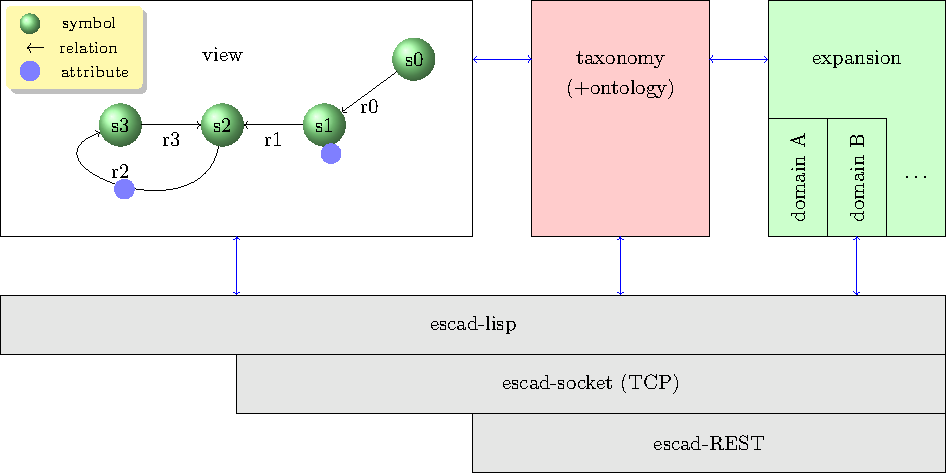
\includegraphics{figures/overview.pdf}
  \caption{Overview of basic escad structure.}
  \label{fig:overview}
\end{figure}
Whenever needed you can add classification info (taxonomy) or functionality (expansion). Mathematically (see also \cite{math:taschenbuch_der_mathematik}) you can see this in equations~\ref{eq:graph}:
\begin{align}
  \label{eq:graph}
  V & = \{s0, s1, s2, s3\} \notag \\
  E & = \{r0, r1, r2, r3\} = \{(s0, s1), (s1, s2), (s2, s3), (s3, s2)\}
\end{align}
You see in math you would need no name for relations, as it are ordered pairs of symbols. Escad wants names for symbols and relations. This is because relations can have some optional properties (symbols too), which you can acess via the relation-name. As convenience you can let escad give you automatic generated names, in case you do not care of the exact name.

You can communicate with escad through common-lisp. This communication can also piped through a local TCP-connection. The REST-API uses this method too. Note that for security reasons you should not make such network-communications over the internet, since escad is not encrypted. However you could use technics like VPN if you want such behaviour.
\subsection{Symbol}
In many papers symbols are also called \index{node}node. However escad has the aim to model things into software. Thus a node is a \emph{variable} for something in our thoughts. A symbol can represent a house, a number, a theory, a joke or whatever you want. This shows the great flexibility of escad. In figure~\ref{fig:overview} symbols are circles with names in it (e.g. s0) which you can name however you want as long it is a unique name in the current graph. In case you do not care, escad can generate a unique name for you.
\subsection{Relation}
Relation or in computer science called \index{edge}edge creates relations between symbols.
\subsection{Attribute}
An \index{attribute}attribute is an \emph{optional} specifier of a symbol/relation. It should be used carefull and not missused as an replacement for a additional symbol. Attributes merely are parameters which give the symbol or relation additional information, mostly needed in conjunction with expansions (e.g. giving a filename to a file-generation expansion).
\subsection{Taxonomy}
With taxonomy you can create in escad a classified specific (domain-based) meaning to your symbols and relations. Depending of the taxonomy there may result different (graphical) output or behaviour (functionality). This may sound clear at first, since without that a computer can not know what a symbol means just by interpreting its name.

However in semantic-knowledge field you may hear often words like \index{ontology}ontology. Strictly spoken a taxonomy is merely a classification of things and terms. Ontology \emph{uses} the taxonomy to capture and represent the meaning of a domain. Since escad is aimed to be a practical tool, it has some domain specific ontologie-knowledge included. This is done by the developers of a escad expansion and you may only effect it with some attributes. If you need a special ontologie you have to search for a expansion that fullfills it, or you have to build your own expansion.
\subsection{Expansion}
Expansions are \emph{ordinary symbols} with a \emph{additional function}, given by assigning a taxonomy and executed via activation of a symbol. Nowadays such easily achivable functionality may be called \index{app}\emph{apps}, who can do various things with your graph. This ranges from graphic output to new generated graph-elements. There are many possibilities and you can even write your own expansion(s). Those programms live in the escad environment and can use the provided feature, even of other expansions. However currently there is only a limited set of expansion, but this could increase in time. Feel free to write a expansion for your domain specific needs.

Table~\ref{tab:expansion_overview} shows the available expansions included in the current version of escad.
\begin{table}[htbp]
\definecolor{light-gray}{gray}{0.9}
\rowcolors{2}{light-gray}{black!20} % alterniert Farbe der Tabellenzeilen
\centering
\begin{tabular}{|p{2.5cm}|p{6cm}|p{5cm}|p{2cm}|}
  \hline
  \textbf{topic} & \textbf{file} & \textbf{description} & \textbf{escad version} \\
  \hline
  3D & \path{3d_expansion.lisp} & Generate 3D files. & 0.2 \\
  \hline
  export & \path{export_expansion.lisp} & Export graph to PDF and SVG. & 0.1 \\
  \hline
  flow & \path{flow_expansion.lisp} & Automates processes in escad. & 0.1 \\
  \hline
  generation & \path{generator_expansion.lisp} & Generate objects in view. & 0.1 \\
  \hline
  import & \path{import_expansion.lisp} & Import graphviz dot-file in view. & 0.1 \\
  \hline
  report & \path{report_expansion.lisp} & Report view to latex and PDF. & 0.1 \\
  \hline
  standard & \path{standard_expansion.lisp} & Provides common useful concepts like sets, checks or canonizing. & 0.1 \\
  \hline
\end{tabular}
\caption{Contained expansions in escad and their functionality.}
\label{tab:expansion_overview}
\end{table}
\chapter{Usage}
Here i assume it is easier to get what escad can do for you, by showing escad in work. Note that the output of the following examples may vary a little at your side (becausse of various reasons), but the basic things should be similar.
\section{Tutorial}
We want now do a short session in escad. After installation go to the escad root directory and start escad by typing in a shell in your terminal:
\shellcmdline{./escad start}{>}
This starts escad REPL (no special arguments given). After loading of common-lisp and escad, you should switch from the common-lisp in the escad namespace:
\lispcmdline{(in-package :escad)}{ESCAD>}
Now you can execute all escad commands directly. To see some possible existing symbols type following escad-command:
\escadcmdline{(ls)}{(``\_escad'' ``\_view'')}\label{ex:ls}\index{command example!ls}
You can read more about this command at page~\pageref{it:ls}. We see two symbols which escad has already created for us. The first symbol can contain settings for our current escad session. The second symbol stands for the current working space we are working. In escad this is called \emph{view} and is just a place where you can work. It can hold graph(s), but does not have to. Escad has two views, you can use (toggle with command \texttt{tv}). But mostly you need just one view.
However we heard that escad has symbols and relations. Lets look at the relations:
\escadcmdline{(lr)}{NIL}\label{ex:lr}\index{command example!lr}
Upps, we get \emph{NIL} which is the lisp way of saying that there is nothing. But that is ok, since we just have not created anything yet. So lets create three symbols:
\escadcmdline{(dolist (name '(``one'' ``two'' nil)) (ns name))}{NIL}\label{ex:ns}\index{command example!ns}
This produces three new symbols, which names we not see because of the \texttt{dolist} nature:
\escadcmdline{(ls)}{(``\_escad'' ``\_view'' ``one'' ``two'' ``s0'')}\index{command example!ls}
The third symbol name \texttt{s0} created escad for us, because we provided \texttt{nil}.
Now lets create a relation:
\escadcmdline{(nr nil ``one'' ``two'')}{``r0''}\label{ex:nr}\index{command example!nr}
Now we got
\escadcmdline{(lr)}{(``r0'')}
Note that you can not insert a new relation or symbol which name already exists.
You now have nearly seen all basic operations in escad. Most functionality can be achieved by this. Instead of learning many new commands, you can use in escad symbols which can also represent actions (e.g. exporting a PDF of your view). But how can you execute such a symbol. This makes the command \emph{as}, which \emph{activates} the given symbol:
\escadcmdline{(as ``s0'')}{(``Documentation text...'')}
You can activate every symbol, but most of them will just print some documentation about themselves, like you have seen in the last command. To get another functionality you have to assign a taxonomy which refers to a expansion. Those expansion is then loaded and executes a defined command (which is defined by the taxonomy).
You can easily add taxonomy to a symbol with add a \emph{property}:
\escadcmdline{(s ``s0'' :taxonomy ``escad.symbol.\_escad.export.pdf'')}{(``s0'')}
If you would activate this smybol now, it would produce a pdf with graphic output of your current view. Because you gave no file-name it would generate some. To give a filename you can add a special attribute-property:
\escadcmdline{(asa ``s0'' '(``filename\_relative'' ``my\_file.pdf''))}{(``my\_file.pdf'')}
Now you should get those pdf-file.
This are the most basic commands you need to know in escad. To get detailed command info use command help:
\escadcmdline{(help-command 'cmd\_name)}{(``Documentation text of cmd\_name...'')}
To get basic help type:
\escadcmdline{(help)}{(``Documentation text...'')}
To list available taxonomies use command \texttt{(lta)}.
\section{User stories (included examples explained)}
To get a fast idea how you should work with escad, please read this section carefully. It gives you general hints how to work, and useful example-patterns to make the theory more clear.
This section is divided in subsections. These come from the basic tasks you can do with escad. In short these are:
\begin{description}
\item[Modeling] is the way you describe escad your topic/task of interest. This is a very important task. If you model something, look at the given examples in the \path{examples} directory. Use the most approbiate taxonomy. Try to think carefully when give attributes! Attributes are meant merely as a data to give details to a symbol (mostly for a expansion-usage). In daily work escad supports you in this topic if you use expansions. Many expansions need a 
\item[Exporting] saves your view in a non-escad format. This is usefull for use your view in other programms.
\item[Importing] allows you to get a view stored in a non-escad format.
\item[Reporting] means to create/process a (new) representation/summary of your view. E.g. your view could be a description of a 3D-modell, and with reporting you could get a 3D-file in X3D-format. A report could also check your view for quality (e.g. if there would occur problems when activate a specific expansion).
\item[Generation] creates new symbols, relations or attributes automatically for you. 
\item[Flow] allows you to automate things in escad without to know how to programm in lisp. This also enables live-expansions which periodically activated generate symbols to reflect the state of a continous process.
\end{description}
\subsection{3D (escad version 0.2)}
Generate 3D-models.
\subsection{Contact tracing (escad version 0.2)}
Tool to provide contact tracing, useful by tracking viral deseases (e.g. corona).
\subsection{Documentation}
Create (technical) documentation in latex or PDF file-format (reporting).
\subsection{Exporting}
In case you can not do some things in escad yet or other tools may do better, you can export your graph. You can export the view to:
\begin{description}
\item[graphviz-dot] is a file format for graphviz, which is powerful in graphically layout and drawing of graphs. Export with a expansion.
\item[SVG] is a vector graphic-format viewable through most modern webbrowsers.
\item[PDF] Export with a expansion.
\item[Mindmap] This creates mindmaps in SVG format. Very usefull to view in a browser and to make your graph visible.
\end{description}
\subsection{Flow}
Note: this is not working yet, because it is in development!
A flow is a graph wich models/automates a process. You can use escad to create a process a user should go through (e.g. a question+answer quiz) or a automation which escad should do for you.
\subsection{Importing graphviz dot}
Because interoperability is important in todays heterogenic software world, there should be a way to get graphs from other software.
Graphviz is powerful in graphically drawing of graphs. You can import those graphs with .dot extension. However only basic functionality of dot is currently supported. Import with a expansion.
\subsection{Learning page (version 0.2)}
Standalone-HTML-javascript learning page generator Note: this is not working yet, because it is in development! You can generate html-pages with integrated javascript functionality to train some excercises, e.g. language learning. It provides motivational intuitive training pages which you can easily generate without html or javascript knowledge. The user has to do excercises and gets result if anwer is correct or not.
\subsection{Lessons learned}
You model e.g. deseases and their dependencies. Then you can try to give symptom(s) and ask for possible cause-tracing.
\subsection{Music/sound creation (version 0.2)}
Todo...
\subsection{Mind-map}
Todo...
\subsection{Modelling}
Modelling semantic graphs is not a easy task. Of course you can make easily symbols and relations, but it heavily depends how you use them. In the past many semantic projects are died or got not very sucessfull used at a wide range. Barry Smith stated some reasons (\url{https://www.youtube.com/watch?v=p0buEjR3t8A}) like silo-syndrome, short-half-life-syndrome and reinvent-the-wheel-syndrome. Nowadays there is a sucessfull example in bioinformatic where to show how genes affect our biology (see BFO-ontology). However even with the best ontology you can have problems, if you not use it properly. To use it you should have a clear knowledge on what the terms mean and how to use.

Such problems may also occur with escad. To improve the situation, escad tries to have many examples for several domains and tasks. The aim is to have enough examples so that you have the possibility to adapt it easily to your needs. I believe it makes more sense to use semantics than to have endless discussions what is the ''correct'' taxonomy/ontology.
\subsection{Pedigree}
Todo...
\subsection{Quiz}
Todo...
\section{Questions}
Note: this is not working yet, because it is in development!
Sometimes questions lead to a fast recognition of a problem or help to understand things better. So lets start asking...
\subsection{Development}
\begin{description}
\item[Can i help develop escad?] Of course. Just contact the developer in github.
\end{description}
\subsection{Usage}
\begin{description}
\item[Is there a difference in the power of the different escad interfaces?] Yes. The most powerful is currently the command line interface. New commands appear first there. However this is no rule. The aim is to keep the functionality equal across the interfaces in a later step.
\item[Why you have choosen common-lisp as the language for escad?] That is a good question. Why not javascript or another more popular language? Well may i ask why not lisp? In fact lisp has a very easy synthax, looks very nice in source code ;-) and for many tasks you need not more than three nested parentheses.
\end{description}
\subsection{Other}
\begin{description}
\item[Is there support for other languages as english?]  No not currently. If you want contribute feel welcome.
\end{description}
\chapter{Reference}
Here you should find the full information to work with escad, such as available commands or interfaces. Also you should get some basic things in order to get the idea in how you can extend escad or help in development.
\section{Commandline LISP-REPL (currently recommended)}\label{sec:cmd_line}
The commandline currently provides the full functionality. This means you got a common-lisp REPL with escad-package loaded. This gives you the full power of common-lisp with the ability of the escad-commands to work with a simple graph environment. To get this commandline go to the escad root directory and start escad-commandline by typing in a shell in your terminal:
\shellcmdline{./escad start terminal}{>}
or because terminal-mode is the default you can also type:
\shellcmdline{./escad start}{>}
Without correct command arguments you get a usage message.
Now you can type in escad commands with a namespace-qualifier, in this case the help command (note the output is here ommitted):
\lispcmdline{(escad:help)}{...}
In order to omitting this namespace just type once:
\lispcmdline{(in-package :escad)}{ESCAD>}
Now you can type just (note the output is here ommitted):
\escadcmdline{(help)}{...}
\subsection{Abbreviations and data structures}
The following table~\ref{tab:cmd_abbreviatons} explains used symbols, abbreviations and the data-structures in the reference.
\begin{table}[htbp]
%\definecolor{light-gray}{gray}{0.9}
%\rowcolors{2}{light-gray}{black!20} % alternates color
\centering
\begin{tabular}{l|p{6cm}|p{6cm}}
  \textbf{pattern} & \textbf{description} & \textbf{example} \\
  \hline
  ATTR & attribute taxonomy string & \texttt{``escad.attribute.author''} \\
  \hline
  (ATTR STRING ...) & attribute taxonomy value list & \texttt{(``escad.attribute.author'' ``Author Name'')} \\
  \hline
  NIL & common lisp nil means not true/done & \texttt{NIL} \\
  \hline
  RN & relation name string & \texttt{``r0''} \\
  \hline
  SN & symbol name string & \texttt{``s0''} \\
  \hline
  STRING & string with unspecified or multiple semantic & \texttt{``a message string...''} \\
  \hline
  VN & view number & \texttt{0} \\
  \hline
  + & previous content can occur at least once or multiple times & \\
  \hline
  * & previous content can occur not or multiple times & \\
  \hline
  ... & previous pattern can be continued & \texttt{(0 1 2 ...)} \\
  \hline
  () & basic common-lisp list & \texttt{(1 ``Hello'')} \\
  \hline
  \lbrack\ \rbrack & optional argument(s) & \texttt{(cmd \lbrack\ \rbrack)} \\
  \hline
  \colorbox{black!20}{function argument} & function argument & \\
  \hline
  \colorbox{green!20}{function result} & function result, multiple values seperated by comma are possible & \\
  \hline
\end{tabular}
\caption{Explained abbreviations and symbols.}
\label{tab:cmd_abbreviatons}
\end{table}
\subsection{Commands}
Note that this list may not be complete yet. To get the most actual overview check the inline documentation.
\begin{description}% \item[$\to$]
\item[\parbox{8.5mm}{as}] \label{it:as} \escadcmd{as}{\lbrack\ SN \rbrack}{STRING}{<a>ctivate <s>ymbol in current view.
What happens depends on the taxonomy of the symbol. Many symbols print out a string as their contents.
Symbols which represent expansions will execute the configured function of the expansion.}
\item[\parbox{8.5mm}{asa}] \label{it:asa} \escadcmd{asa}{SN (ATTR STRING ...)+}{SN | NIL}{
<A>dd/edit <s>ymbol <a>ttributes depending of key. NIL if nothing is added.}
\item[\parbox{8.5mm}{gra}] \label{it:gra} \escadcmd{gra}{RN attribute-string}{STRING}{<G>et <r>elation <a>ttributes depending of given attribute-string.}
\item[\parbox{8.5mm}{gsa}] \label{it:gsa} \escadcmd{gsa}{SN attribute-string}{STRING}{<G>et <s>ymbol <a>ttributes depending of given attribute-string.}
\item[\parbox{8.5mm}{help}] \label{it:help} \escadcmd{help}{}{STRING}{Print <help>ful overview of escad, meaning of terms and all available commands.}
\item[\parbox{8.5mm}{lr}] \label{it:lr} \escadcmd{lr}{\lbrack\ :filter :exclude-taxonomy \rbrack}{(RN*)}{<L>ist all <r>elations in current schematic which name match the filter. Additionally exclude relations which match the exclude-taxonomy.}
\item[\parbox{8.5mm}{ls}] \label{it:ls} \escadcmd{ls}{\lbrack\ :filter :exclude-taxonomy \rbrack}{(SN*)}{<L>ist all <s>ymbols in current schematic which name match the filter. Additionally exclude symbols which match the exclude-taxonomy.} See example at page~\pageref{ex:ls} for usage.
\item[\parbox{8.5mm}{nr}] \label{it:nr} \escadcmd{nr}{RN | nil SN SN \lbrack\ :attributes :comment :taxonomy :weight \rbrack}{RN | nil}{Create <n>ew <r>elation with given name and possible additional values in view. If the relation-name already exists do nothing and return nil. Default type is undirected relation. To make a directed or bidirected relation, set the appropriate taxonomy (note that ref\_from and ref\_to are only technical terms meaning you first tie the relation from that symbol to another. it can mean that is directe, but it is not guaranted that the author means that unless he makes that explicit with a relation that declares that).}
\item[\parbox{8.5mm}{ns}] \label{it:ns} \escadcmd{ns}{SN | nil \lbrack\ :attributes :comment :taxonomy :weight \rbrack}{SN | nil}{Create <n>ew <s>ymbol with given name and possible additional values in view. If the symbol-name already exists do nothing and return nil.}
\item[\parbox{8.5mm}{r}] \label{it:r} \escadcmd{r}{RN \lbrack\ :comment :ref\_from :ref\_to :taxonomy :weight \rbrack}{RO | nil}{Get/set <r>elation object.}
\item[\parbox{8.5mm}{s}] \label{it:s} \escadcmd{s}{SN \lbrack\ :comment :taxonomy :weight \rbrack}{SO | nil}{Get/set <s>ymbol object.}
\item[\parbox{8.5mm}{tv}] \label{it:tv} \escadcmd{tv}{}{VN}{<T>oggle <v>iew since escad has two views change from the one to the other and gives back the number of the new view (0 or 1).}
\item[\parbox{8.5mm}{vs}] \label{it:vs} \escadcmd{vs}{}{(VN SC1 RC1 SC2 RC2)}{Gives <v>iew <s>tatus.}
\end{description}
\section{Emacs with LISP-REPL and view buffer}
This is currently possible for experienced users via slime-mode in emacs.
\section{Tk GUI}
This is in development but currently in sleep, because other user interfaces are prefered.
\section{TCP-Socket}
This section can refer fully to section~\ref{sec:cmd_line}. The same commands are available, except that they are transmitted via TCP-Socket as a text-stream. However it is \emph{not} intended to acess over external network, instead you should use it locally. If you need external acess use virtual private networks or the REST-API.
\section{REST-API}
This is in development. The API is especially meant for a structured and safe acess to escad without the possibility to execute (potential more powerful/dangerous) lisp commands. Additionally the REST-API (even if it is not a standard in itself) uses standards such as HTTP, URI and JSON. With the paradigm CRUD (create, read, update, delete) there is for the user a clear set of actions available, which can be used on the objects in a view. HATEOAS (Hypermedia as the Engine of Application State) allows the consuming applications a guided way through the complexity of a graph.
\section{Library}
To use escad as a library in your common lisp programm, just load \path{package.lisp}.
\section{HTML-client}
This is in development and not fully working yet.
\section{Included expansions}
Those are the expansions which are included/shipped in this escad-package. Note that currently this part is less actual, since we first want concentrate on the big picture - before diving in the details. However details can be documented in parts which are relatively mature.
\subsection{export\_expansion.lisp}
The following table~\ref{tab:exp-export-expansion} explains the export expansion.
\newcommand{\tabitem}{~~\llap{\textbullet}~~}
\begin{table}[htbp]
\centering
\begin{tabular}{r|p{11cm}}
  \textbf{taxonomy} & \colorbox{black!20}{escad.symbol.\_escad.export.dot} \\
  \hline
  \textbf{in} & - \\
  \hline
  \textbf{out} & - \\
  \hline
  \textbf{attribute} & 1. symbol name \\
                     & 2. [file name] \\
  \hline
  \textbf{description} & exports view to dot (graphviz) \\
  \hline
  \hline
  \textbf{taxonomy} & \colorbox{black!20}{escad.symbol.\_escad.export.pdf} \\
  \hline
  \textbf{in} & - \\
  \hline
  \textbf{out} & - \\
  \hline
  \textbf{attribute} & 1. symbol name \\
                     & 2. [file name] \\
  \hline
  \textbf{description} & exports view to pdf \\
  \hline
  \hline
  \textbf{taxonomy} & \colorbox{black!20}{escad.symbol.\_escad.export.svg} \\
  \hline
  \textbf{in} & - \\
  \hline
  \textbf{out} & - \\
  \hline
  \textbf{attribute} & 1. symbol name \\
                     & 2. [file name] \\
  \hline
  \textbf{description} & exports view to svg. \\
\end{tabular}
\caption{Symbols and relations of export expansion.}
\label{tab:exp-export-expansion}
\end{table}
\chapter{Development}
Everyone is needed and welcome for escad development. If you are a graphical designer, you are got in documenting or you like to program in lisp or you are interested in web-programming - all is required in escad. :-)
The project is managed with the famous source-code management tool \emph{git} (also known as used in the linux kernel development). The repository is hosted under \url{https://github.com/mkollmar/escad}.
\section{Directory structure}
The directory structure of the repository will be explained in this section. This structure also mirrors the different workflows which exist.
\subsection{doc/*}
Contains like the name says the escad documentation. Currently this is mainly this manual written in \emph{latex}. But in future a unix man-page, more examples or online documentation would be great, too.
The compilation of this latex-document can be done with the command \shellcmdline{latexmk}{>}. \path{doc/figures} contains figures needed for the manual. Those will be compiled if needed automatically via \emph{latexmk}.
\subsection{examples/*}
\path{examples} contains examples which can be loaded in escad. But note that currently not all may work yet, they are more a print what a future interface should look like.
\subsection{lib/*}
\path{lib} contains the escad-lisp files.
\subsection{node\_modules/*}
\path{node\_modules} contains the code-modules for node.js. Some functions are written for node (a javascript execution environment, similar the one in your browser). The REST-server is a example that needs node.
\subsection{public/*}
\path{public} contains the files which are accesible via web by the REST-server.
\subsection{test/*}
\path{test} is needed for development to test current implementation if it fullfills the requirements/functions needed.
\subsection{ui/*}
\path{ui} contains files needed for the various user interfaces that escad may support now or in future.
\section{Programming your own expansion}
Writing escad expansions is not difficult. Go through following steps carefully and you will have a good basis for writing your own. The code in listing~\ref{listing:exp_minimal} shows a minimal expansion and the listing~\ref{listing:exp_tax} shows the entry in a taxonomy file.
\begin{lstlisting}[caption={Minimal expansion code.}, language=Lisp, morekeywords={in-package, use}, label=listing:exp_minimal]
(in-package "COMMON-LISP-USER")
(defpackage :de.markus-herbert-kollmar.escad.expansion.hello_world
  (:use :common-lisp :escad)
  (:export :my-function)
  (:documentation "This is my expansion which does nothing usefull."))
(in-package :de.markus-herbert-kollmar.escad.expansion.hello_world)
(defun my-function (symbol-name-string)
"This function will be executed by calling this expansion.")
\end{lstlisting}
\begin{lstlisting}[caption={Entry in a taxonomy-file.}, language=Lisp, morekeywords={}, label=listing:exp_tax]
(:taxonomy "escad.symbol.hello_world" :doc "[E] Hello world."
:expansion "hello_world_expansion.lisp"
:package :de.markus-herbert-kollmar.escad.hello_world
:function "my_function"
:license "GNU GPL 3")
\end{lstlisting}
Following things you should keep in mind:
\begin{itemize}
\item Choose namespace.
\item Provide documentation within your expansion.
\item Provide at least one function which can be called with the symbol-name-string as first argument und some possible further arguments.
\item Provide a taxonomy file with your expansion declaration or request that your expansion will be taken into the default escad-taxonomy.
\end{itemize}
You are wellcome if you want include your expansion in this escad distribution.

\clearpage % newpage allows to let appear figures after creating new page.
%\newpage

%%%%%%%%%%%%%%%%%%%%%%%%%%% BIBLIOGRAPHY
% \bibliographystyle{plain}
\printindex
\bibliographystyle{alpha}
\bibliography{bibliography}

\end{document}
